\chapter{Complejidad: Notaci\'on asint\'otica}

La principal motivaci\'on para usar la complejidad es poder comparar algoritmos, particultarmente para problemas grande (para los m\'as chicos no es tan importante). Es por esto que utilizamos la notaci\'on asint\'otica, que consiste en observar a una funci\'on cuando su dominio (el tama\~no del problema) tiende a infinito. Como la funci\'on de complejidad depende del tama\~no del problema, agruparemos las instancias de acuerdo a este parametro. Sin embargo, distintas instancias con el mismo tama\~no pueden llegar a comportarse de maneras muy diferentes. Es por esto que al analizar el algoritmo separamos el an\'alisis en mejor caso, peor caso y caso promedio.

Las notaciones que usamos para describir la complejidad temporal asint\'otica de un algoritmo est\'an definidos en t\'erminos de funciones cuyos dominios son el conjunto de los n\'umeros naturales $N = \{0,1,2,...\}$. Estas notaciones son convenientes para describir el tiempo en el peor caso de una funci\'on $T(n)$, la cual usualmente esta definida solo en tama\~nos de entrada enteros. Usaremos la notaci\'on asint\'otica primariamente para describir los tiempos que insumen los algoritmos; sin embargo, se aplica a las funciones en general. La notaci\'on asint\'otica permite abstraerse de los detalle de la funci\'on en s\'i y tener una noci\'on aproximada, m\'as simplificada.

\begin{SCfigure}[1][ht!]
 \centering
 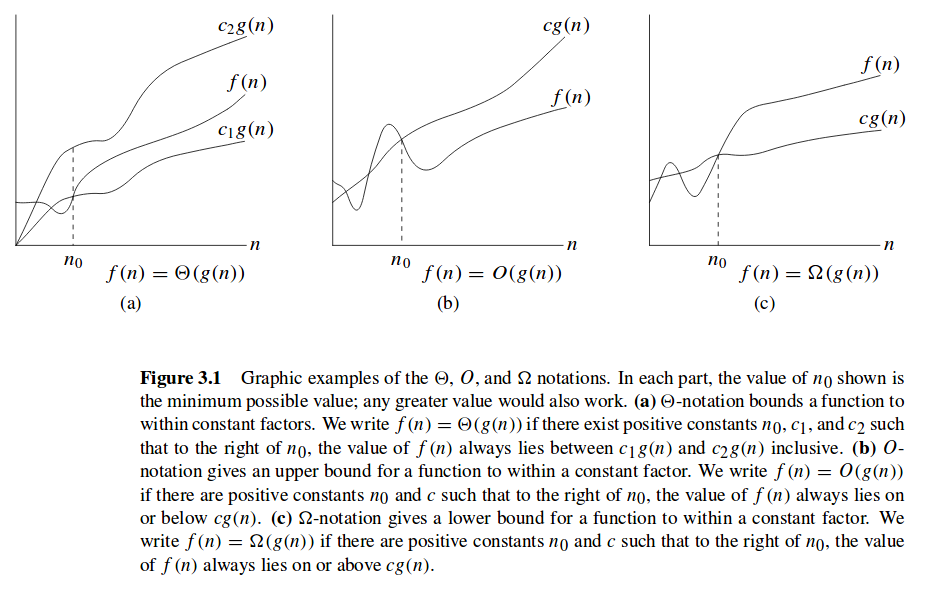
\includegraphics[width=0.9\textwidth]{graficos/complejidad.png}
\end{SCfigure}

\section{Notaci\'on $\Theta$}

Para una funci\'on $g(n)$ dada, notaremos a $\Theta(g(n))$ como el conjunto de funciones $f(n)$ que a partir de un numero $n_0 > 0$ sus valores pueden ser acotados entre $c_1g(n)$ y $c_2g(n)$ para alg\'un $c_1, c_2 \in \Re_{>0}$. Descripto formalmente quedar\'ia de la siguiente manera:

\begin{equation*}
 \Theta(g(n)) = \{ f(n) : (\exists\ c_1, c_2, n_0 \in \Re_{>0}) \ (\forall n\ |\ n_0 \leq n)\ 0 \leq c_1 \cdot g(n) \leq f(n) \leq c_2 \cdot g(n) \}
\end{equation*}

~

Como $\Theta(g(n))$ es un conjunto, podremos escribir ``$f(n) \in \Theta(g(n))$'' para indicar que $f(n)$ es un miembro de $\Theta(g(n))$, a veces escribiremos ``$f(n) = \Theta(g(n))$'' para expresar exactamente lo mismo.
~

\textbf{Propiedades de $\Theta$}:
\begin{enumerate}
 \item Para cualquier funci\'on $f$ se tiene que $f \in \Theta(f)$.
 \item $\Theta(f) = \Theta(g) \iff f \in \Theta(g) \iff g \in \Theta(f)$.
 \item S\'i $f \in \Theta(g) \land g \in \Theta(h) \implies f \in \Theta(h)$.
 \item S\'i $f \in \Theta(g) \land f \in \Theta(h) \implies \Theta(g) = \Theta(h)$.
 \item S\'i existe $\lim_{n \to \infty} \frac{f(n)}{g(n)} = k$, seg\'un los valores que tome $k$:
	\begin{enumerate}
	  \item S\'i $k \neq 0$ y $k < \infty$ entonces $\Theta(f) = \Theta(g)$.
	  \item S\'i $k = 0$ entonces $\Theta(g) \neq \Theta(f)$.
	\end{enumerate}
\end{enumerate}

\section{Notaci\'on $O$}

El conjunto $\Theta$ asint\'oticamente acota una funci\'on inferior y superiormente. Cuando solo tenemos una \textbf{cota asint\'otica superior}, usaremos el conjunto $O$. Para una funci\'on dada $g(n)$, denotaremos por $O(g(n))$ al conjunto de funciones tales que:

\begin{equation*}
 O(g(n)) = \{ f(n) : (\exists\ c, n_0 \in \Re_{>0}) \ (\forall n\ |\ n_0 \leq n)\ 0 \leq f(n) \leq c \cdot g(n) \}
\end{equation*}

~

Es decir que para todos los valores de $n$ a la derecha de $n_0$, el valor de la funci\'on $f(n)$ est\'a por debajo de $c \cdot g(n)$. Escribiremos $f(n) = O(g(n))$ para indicar que una funci\'on $f(n)$ es un miembro del conjunto $O(g(n))$. Notar que $f(n) = \Theta(g(n))$ implica $f(n) = O(g(n))$, ya que la noci\'on de $\Theta$ es mucho mas fuerte que la noci\'on de $O$. Esto es, escrito en forma de teor\'ia de conjuntos, que vale la inclusi\'on $\Theta(g(n)) \subseteq O(g(n))$

~

\textbf{Propiedades de $O$}:
\begin{enumerate}
 \item Para cualquier funci\'on $f$ se tiene que $f \in O(f)$.
 \item $f \in O(g) \implies O(f) \subset O(g)$.
 \item $O(f) = O(g) \iff f \in O(g) \land g \in O(f)$.
 \item S\'i $f \in O(g) \land g \in O(h) \implies f \in O(h)$.
 \item S\'i $f \in O(g) \land f \in O(h) \implies f \in O(min(g,h))$.
 \item S\'i existe $\lim_{n \to \infty} \frac{f(n)}{g(n)} = k$, seg\'un los valores que tome $k$:
	\begin{enumerate}
	  \item S\'i $k \neq 0$ y $k < \infty$ entonces $O(f) = O(g)$.
	  \item S\'i $k = 0$ entonces $f \in O(g)$, es decir, $O(f) \subset O(g)$, pero sin embargo se verifica que $g \notin O(f)$.
	\end{enumerate}
\end{enumerate}

\section{Notaci\'on $\Omega$}

De forma tal como la notaci\'on $O$ proporciona una cota asint\'otica en una funci\'on, $\Omega$ provee una \textbf{cota asint\'otica inferior}. Para una funci\'on dada $g(n)$, notaremos a $\Omega(g(n))$ como el conjunto de funciones tales que:

\begin{equation*}
 \Omega(g(n)) = \{ f(n) : (\exists\ c n_0 \in \Re_{>0}) \ (\forall n\ |\ n_0 \leq n)\ 0 \leq c \cdot g(n) \leq f(n) \}
\end{equation*}

~

Cuando decimos que el tiempo de un algoritmo es $\Omega(g(n))$, significa que no importa que particular entrada de tama\~no $n$ para cada valor de $n$, el tiempo que tardara el algoritmo con dicha entrara sera de al menos un numero constante de veces $g(n)$, para un $n$ suficientemente grande. Equivalentemente, esto nos da una cota temporal inferior para el mejor caso del algoritmo. De las definiciones de las notaciones asint\'oticas, es f\'acil ver que para cualquier dos funciones $f(n)$ y $g(n)$, tendremos que $f(n) = \Theta(g(n))$ si y solo si $f(n) = O(g(n))$ y $f(n) = \Omega(g(n))$. Usando una notaci\'on de teor\'ia de conjuntos esto seria equivalente a decir que $\Omega(g(n)) \cap O(g(n)) = \Theta(g(n))$, y si $f(n) \in \Omega(g(n)) \land f \in O(g(n))$ entonces $f(n)$ pertenecer\'a a ambos conjuntos, por lo que en particular pertenecer\'a a la intersecci\'on $\Theta(g(n))$.

~

\textbf{Propiedades de $\Omega$}:
\begin{enumerate}
 \item Para cualquier funci\'on $f$ se tiene que $f \in \Omega(f)$.
 \item $f \in \Omega(g) \implies \Omega(f) \subset \Omega(g)$.
 \item $\Omega(f) = \Omega(g) \iff f \in \Omega(g) \land g \in \Omega(f)$.
 \item S\'i $f \in \Omega(g) \land g \in \Omega(h) \implies f \in \Omega(h)$.
 \item S\'i $f \in \Omega(g) \land f \in \Omega(h) \implies f \in \Omega(max(g,h))$.
 \item $f(n) = \Omega(g(n)) \iff g(n) = O(f(n))$
 \item S\'i existe $\lim_{n \to \infty} \frac{f(n)}{g(n)} = k$, seg\'un los valores que tome $k$:
	\begin{enumerate}
	  \item S\'i $k \neq 0$ y $k < \infty$ entonces $\Omega(f) = \Omega(g)$.
	  \item S\'i $k = 0$ entonces $g \in \Omega(f)$, es decir, $\Omega(g) \subset \Omega(f)$, pero sin embargo se verifica que $g \notin \Omega(f)$.
	\end{enumerate}
\end{enumerate}

\textbf{Teorema:}
Para dos funciones cualesquiera f(n) y g(n), $f(n)= \Theta(g(n))$ si y solo si $f(n)= O(g(n))$ y $f(n)= \Omega(g(n))$
